

\documentclass[conference]{IEEEtran}

\usepackage{graphicx,color}
\ifCLASSINFOpdf
  % \usepackage[pdftex]{graphicx}
  % declare the path(s) where your graphic files are
  % \graphicspath{{../pdf/}{../jpeg/}}
  % and their extensions so you won't have to specify these with
  % every instance of \includegraphics
  % \DeclareGraphicsExtensions{.pdf,.jpeg,.png}
\else
  % or other class option (dvipsone, dvipdf, if not using dvips). graphicx
  % will default to the driver specified in the system graphics.cfg if no
  % driver is specified.
  % \usepackage[dvips]{graphicx}
  % declare the path(s) where your graphic files are
  % \graphicspath{{../eps/}}
  % and their extensions so you won't have to specify these with
  % every instance of \includegraphics
  % \DeclareGraphicsExtensions{.eps}
\fi



% correct bad hyphenation here
\hyphenation{op-tical net-works semi-conduc-tor}


\begin{document}

\title{Planning Paths for Rats using Actor-Critic Model}


\author{Zachary DeStefano}

% make the title area
\maketitle


\begin{abstract}
For this project, I attempted to see what paths a rat would take if the Morris Water Maze contained multiple rewards of varying value. The inspiration for this project was the layout of cities and the transportation networks used to connect them. I hoped to observe if a trained rat would use paths that look similar to those transportation networks. In order to do this, I trained the rat using hippocampal place cells that learn via temporal difference learning in the actor-critic model. After training, I started the rat at random locations and recorded the paths it took to the reward centers. In the end, the paths are suboptimal thus rats should not be used for path planning. 
\end{abstract}

\IEEEpeerreviewmaketitle



\section{Introduction}

The Morris Water Maze is one where a rat is released into a pool of water and searches for a platform which will provide relief from having to swim. The platform is thus considered a reward in the brain of the rat. Due to the constant location of these platforms, it is optimal for the rat to learn this location. By observing the rat over multiple trials we can extrapolate information about its learning abilities.\\
\\
If we wish to approximate what would happen if we did a physical experiment, we can use a model for its neuronal activity. For the purposes of this experiment, I assumed that there are a series of place cells in its hippocampus that each have their own actor and critic cells. The place cells fire at their own preferred locations and send signals to the actor and critic cells. When the rewards are reached, the actor and critic values are updated using the Temporal Difference learning rule. Output from the actor and critic cells is used to determined the rat's next move. The neuronal network described was implemented by Foster et all **CITE PAPER**. \\
\\
In the paper by Foster, they had a single reward center for the rat. For this experiment, I wanted to observe what could happen if you used the same neuron model but had multiple reward centers. More specifically, I wanted to observe the paths that a rat would take to travel between all the reward centers. The hope is that something similar to a Steiner Tree **INSERT CITATION** would emerge. 

\section{Related Work}

\subsection{Steiner Tree Problem}

The Euclidean Steiner Tree Problem is as follows: Given $n$ points in a $2D$ plane, connect them via line segments such that the total line segment length is minimized and every point can travel to every other point. Currently this problem is NP-hard meaning that it is not known whether or not there is an efficient algorithm. There is a polynomial time approximation scheme that has been found for it **INSERT CITATION**.  

\subsection{Slime Mode Interstates}

There was an attempt at solving something similar to the Steiner Tree problem using the behavior of biological organisms. Food was placed at locations imitating the 20 largest cities in the United States and then slime mold was released. **INSERT CITATION** The paths sketched out by the slime mold ended up being similar to the interstate highway system and is thus likely similar to what the Steiner Tree would look like. This is a great example of how the aggregate of simple actions taken by a biological organism can yield useful results. My goal with the rat experiment was to see if we would get useful results taking the aggregate of the paths it takes after learning. 

\subsection{DA-STDP for foraging tasks}

Another model that has been proposed in the literature to simulate reinforcement learning is Dopamine-modulated Spike-time dependent plasticity (DA-STDP). There are two papers in particular where they used it to model a direct actor foraging for rewards. \\
\\
In a paper by Skorkheim et al **PLOS ONE PAPER**, they model an actor foraging for food using DA-STDP. As it turns out, DA-STDP can be used to model the behavior effectively, however you have to impose additional constraints related to maintaining synaptic homeostasis in order for it to be effective. A similar experiment was done by Evans et al **ROBOT PAPER**, where he modeled the movement of a robot foraging for food in an environment. \\
\\
These papers indicate that it may be possible to use DA-STDP to model the rat's behavior in my environment. However, there are two key differences between my set-up and those papers. First, in my experiment, the input is place cells thus the rat knows its global location. In those papers, the input is the immediate environment around the actor at a given point. The second major difference is that both experiments have many food items spread around the environment and it does not matter which food items the actor receives. For my experiment, I only had a few reward centers and I was aiming for the actor to visit all of them. 



\section{Experiment Design}

\subsection{Rat Movements}

For the real experiments there would be a rat moving around a circular pool. I thus had a "rat" with an x-y location moving around a circle. In my model, the rat has place cells in its hippo-campus and each of the place cells has a preferred location in the circle. Each place cell feeds into a critic cell as well as 8 actor cells. The place cell location, responses by the actor and critic cells, and final direction chosen by the rat was determined using the model specified in Foster et al **INSERT CITATION**. \\
\\
There were two important things to consider when modeling the rat's movements: how much it changes direction and what to do if it hits the wall. For simplification, I assumed that a rat "bounces off" a wall if it hits it. This means that I had $\pi$ radians to its direction of movement in order to reverse it. When doing this, it is possible that if the rat hits the wall from a certain angle and is at the right location, then it could keep bouncing forever. **INSERT PICTURE**. If the rat failed to be at a proper location after "bouncing" then I change its direction by $\frac{\pi}{2}$ radians in order to prevent this from occurring. \\
\\
The other thing to consider is how much the rat's direction is allowed to change in each time step. Here I deviated from the design in Foster **INSERT CITATION** and chose my own method. I assumed that in each time step, the rat has only three choices: continue traveling in the same direction, move slightly to the left, or move slightly to right. Traveling in the same direction means that the angle of movement stays constant. Moving slightly to the left means that the angle increases by $\frac{\pi}{4}$ radians. Moving slightly to the right means the angle decreases by $\frac{\pi}{4}$ radians. In order to determine the rat's next move, I shifted the coordinate system so that the previous angle was the positive x-direction. If the vector representing the next angle had a positive y-value then I had the rat move slightly to the left. If the vector had a negative y-value then the rat moved slightly to the right.

\subsection{Rat Training and Rewards}

In order to train the rat, I followed the procedure used in Foster **INSERT CITATION** and used many parts of the morris\_water\_maze.m code. In each trial, the rat was released in one of 4 locations and then "moved" (as described above) until it found a reward center or 250 time steps had passed, whichever came first. Once the reward center was found, the actor critic values were updated. Unlike in Foster **INSERT CITATION**, I had multiple reward centers. Initially they all gave a reward of 1.\\
\\
In order to make sure a rat does not get too attached to one reward, their reward value decreased by a constant amount each time the rat reached it. The reward center was not used once the value fell below a certain threshold. The rat was trained until a certain number of trials occurred or all the rewards had been spent, whichever came first. \\
\\
In order to see if there would be an effect if we modeled the fact that cities have different populations, I also ran trials where the initial reward values were different **IMPLEMENT THIS AND SHOW FIGURES**. I took the population values and did a rescale and shift so that they fell between 0.5 and 1. 

\subsection{Reward Center Locations}
For the reward center locations, I used basic locations to start off and then used locations inspired by the cities in the United States and Europe. \\
\\
In order to have well placed cities, for my United States map, I used New York, Chicago, Los Angeles, Atlanta, and Denver. For the Europe map, I used Paris, London, Warsaw, Berlin, and Vienna. I found their latitude and longitude coordinates in signed degrees format and plotted them on a 2D plane, rescaling for the water maze. I made sure to vary which particular set of cities I chose in a given trial. 

\subsection{Rat Testing}

Once the rat was trained, I recorded the paths it takes when released back into the maze. The rat movement was exactly the same as during training except that the actor and critic values were left unchanged. The rat also started at random locations in the maze. In order to model a random location, I used polar coordinates and chose random $\theta$ and $r$ values that are within the realm of the circle and then converted the $(r,\theta)$ pair to its corresponding $(x,y)$ pair. 
**MENTION THAT RAT MIGHT NOT STOP AT REWARD CENTERS**


\section{Results}

One of the tradeoffs was that without sufficient training, the rat tends to hang around areas that are at an equal distance from the reward centers and cannot decide which direction to go in. \\
\\
FIGURES WITH THE PATH RESULTS AND LEARNED ACTOR-CRITIC VALUES\\
INCLUDE FIGURES SHOWING CUMULATIVE DISTANCE TO THE TARGET\\
\\
It can be reasonably assumed that the highest capacity highway would need to be placed where the rat's activity is the greatest. Indeed, the region with a high amount of activity is around the center of the city points. \\
\\
For figure **INSERT REF**, I used the cities of Berlin, Vienna, and Warsaw as my model for the reward center locations. During the testing phase, the rat moves toward one of the cities and also travels around the area between the cities. The interesting thing is that if you take the areas in the figure where the path lines are densest, then it could almost make a path that would make sense as travel routes between the cities. 
**MENTION DEPRECIATION METHOD USED FOR THIS ONE**

\begin{figure}
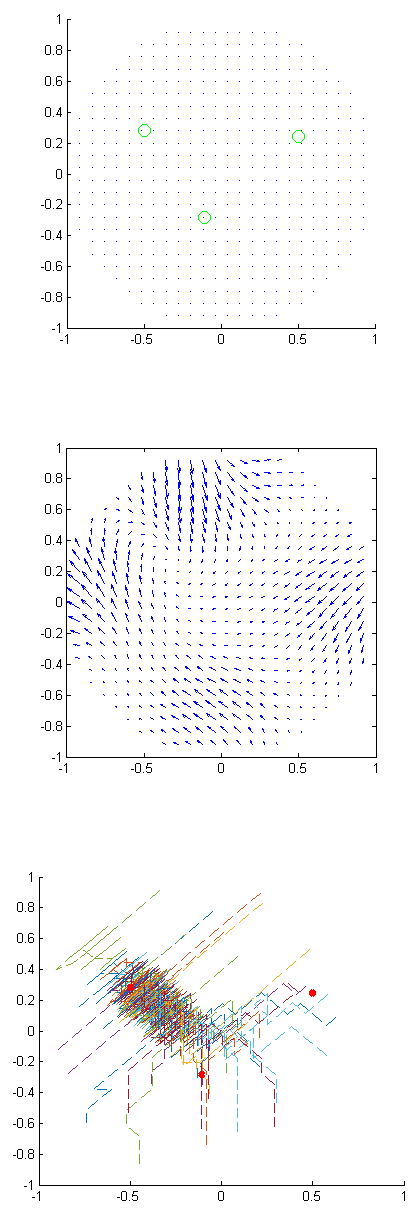
\includegraphics[width=0.4\textwidth]{waterMazeRevised2_Figure.png} 
\caption{Place Cell and Reward Center Locations (top). Actor Gradient (middle). Paths traversed by rat with reward centers in red (bottom)}
\end{figure}

\begin{figure}
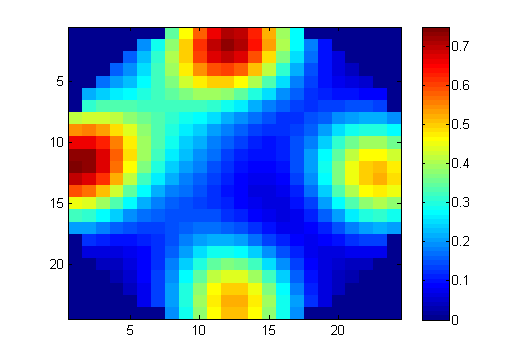
\includegraphics[width=0.4\textwidth]{waterMazeRevised2_Critic.png} 
\caption{Critic Values in Maze}
\end{figure}

For figure **INSERT REF**, I used the cities of New York, Chicago, Los Angeles, Seattle, and Atlanta. After training, the rat had relatively good actor gradient directions. When charting all the paths the rat took, there is a high density in the middle area between all the cities which would coincide with where we would want a road to be to go between all the cities. 

\begin{figure}
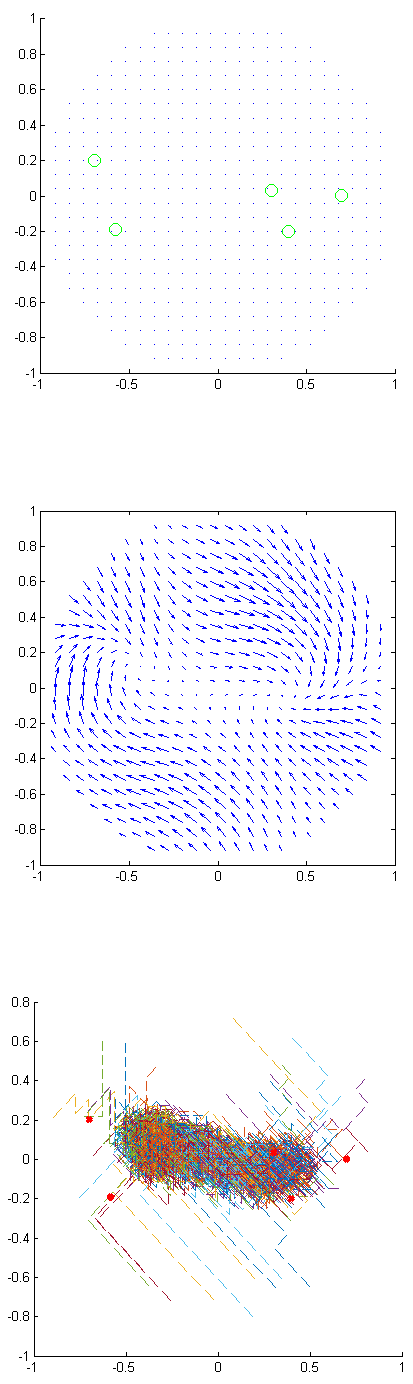
\includegraphics[width=0.4\textwidth]{waterMazeRevisedD_Figure.png} 
\caption{Place Cell and Reward Center Locations (top). Actor Gradient (middle). Paths traversed by rat with reward centers in red (bottom)}
\end{figure}

\begin{figure}
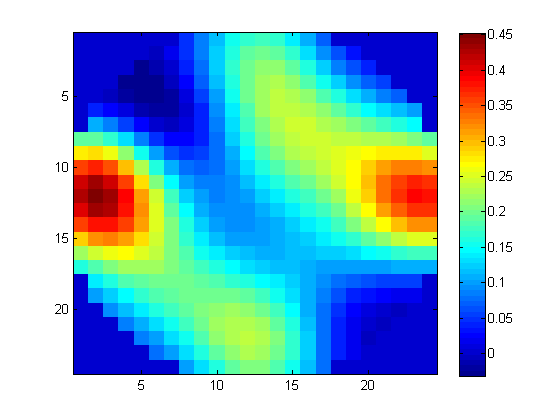
\includegraphics[width=0.4\textwidth]{waterMazeRevisedD_Critic.png} 
\caption{Critic Values in Maze}
\end{figure}

For figures **INSERT REF**, I used the European cities but changed their initial reward values based on their population. 

\begin{figure}
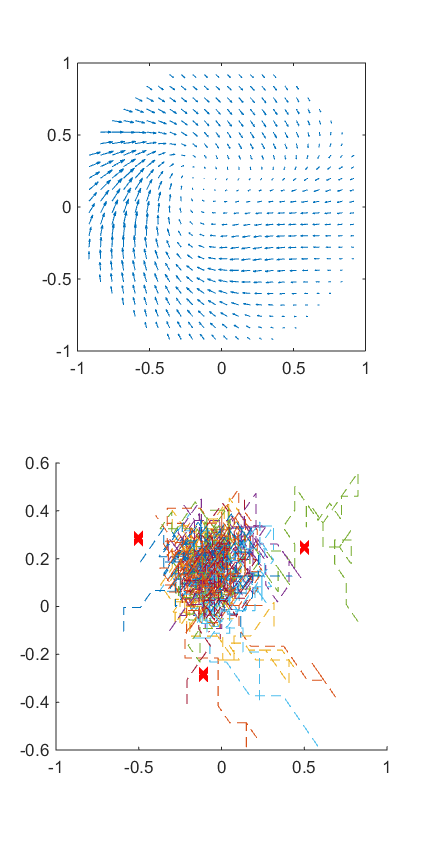
\includegraphics[width=0.4\textwidth]{waterMazeRevised2_Figure_populationRewards.png} 
\caption{Place Cell and Reward Center Locations (top). Actor Gradient (middle). Paths traversed by rat with reward centers in red (bottom)}
\end{figure}

\begin{figure}
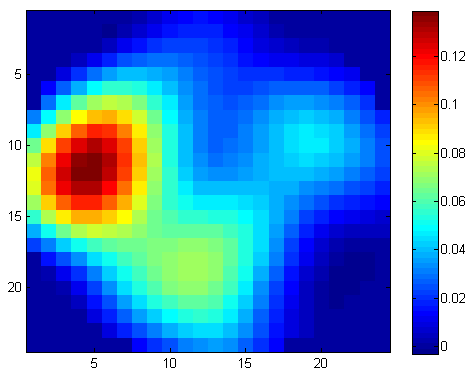
\includegraphics[width=0.4\textwidth]{waterMazeRevised2_Critic_populationRewards.png} 
\caption{Critic Values in Maze}
\end{figure}

For figures **INSERT REF**, I used the American cities but changed their initial reward values based on their population. 

\begin{figure}
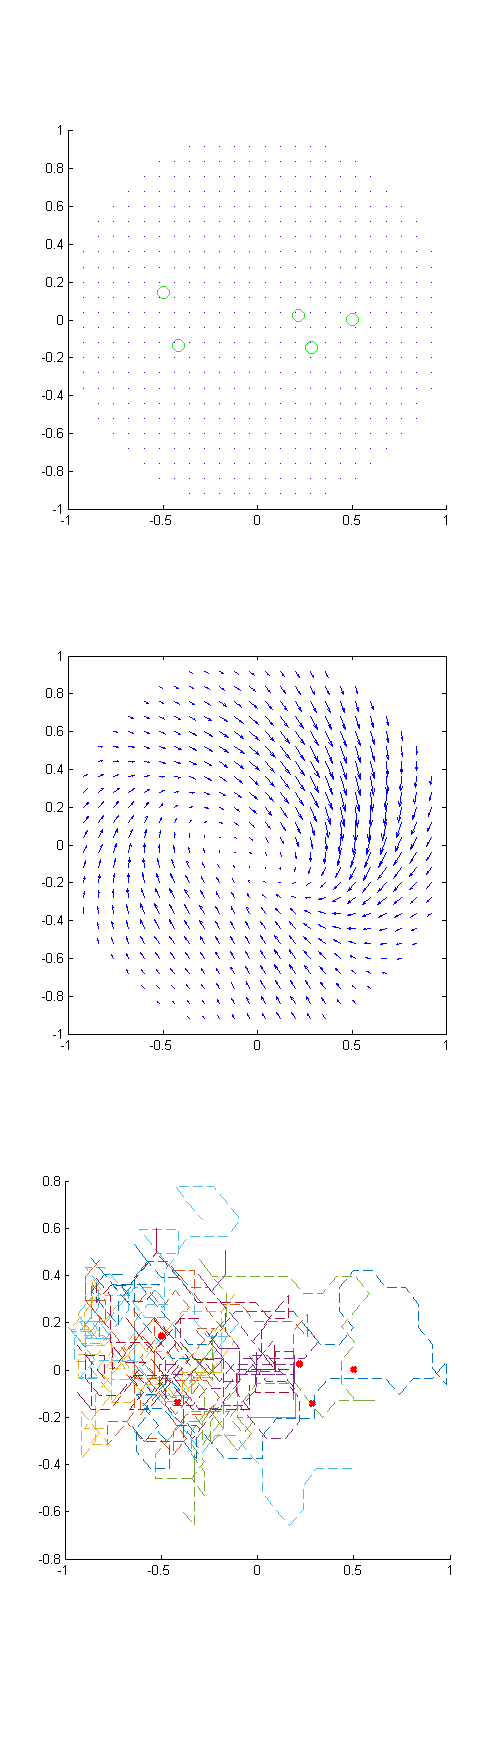
\includegraphics[width=0.4\textwidth]{waterMazeRevisedD_Figure_populationRewards.png} 
\caption{Place Cell and Reward Center Locations (top). Actor Gradient (middle). Paths traversed by rat with reward centers in red (bottom)}
\end{figure}

\begin{figure}
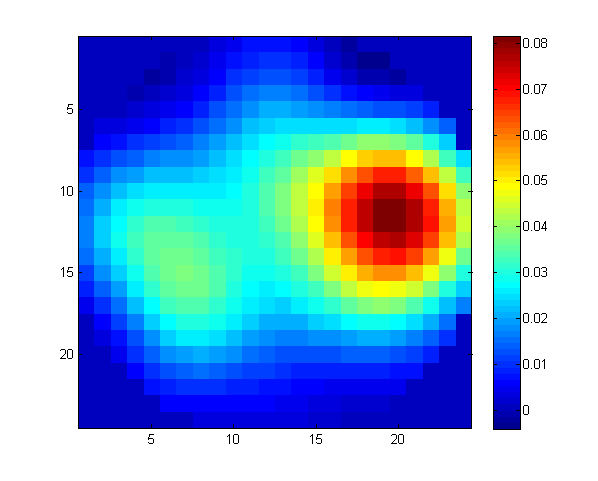
\includegraphics[width=0.4\textwidth]{waterMazeRevisedD_Critic_populationRewards.png} 
\caption{Critic Values in Maze}
\end{figure}

\section{Conclusion}
Rats should not be used for path planning. It was quite difficult getting the model to overcome adverse behaviors and even then, the paths taken were not terribly informative. Additionally, more efficient paths could easily be found. The hope with this project was that the actor-critic model would find compromise directions for each place cell and after enough training, you could use the actor cells to map out efficient paths all around the maze, either to the cities or between cities. \\
\\
Other things should be used for the Steiner Tree Problem. \\
\\
In all likelihood, the actor-critic model is not well suited for multiple objects and definitely not the Steiner Tree issue. \\
\\

\section{Future Work}

The lack of reward centers would make it difficult to model the spiking in a DA-STDP model, but still possible. The input would be the place cell activity and it would connect to a network of excitatory and inhibitory networks modulated by DA-STDP. The output from these neurons could be used to determine the next move for the rat. This network would be extremely similar to the one presented in the **PLOS ONE PAPER** with the main difference being the input layer. 

The lack of reward centers in my experiment would mean that there would be relatively little spiking in a DA-STDP model thus it would be difficult to obtain the behavior I would want. 

\begin{thebibliography}{1}

\bibitem{IEEEhowto:kopka}
H.~Kopka and P.~W. Daly, \emph{A Guide to \LaTeX}, 3rd~ed.\hskip 1em plus
  0.5em minus 0.4em\relax Harlow, England: Addison-Wesley, 1999.

\end{thebibliography}




% that's all folks
\end{document}


